%\documentclass[mat1]{fmfdelo}
% \documentclass[fin1]{fmfdelo}
% \documentclass[isrm1]{fmfdelo}
 \documentclass[mat2]{fmfdelo}
% \documentclass[fin2]{fmfdelo}
% \documentclass[isrm2]{fmfdelo}

% naslednje ukaze ustrezno napolnite
\avtor{Tom Gornik}

\naslov{Izrek Šarkovskega}
\title{Sharkovsky theorem}

% navedite ime mentorja s polnim nazivom: doc.~dr.~Ime Priimek,
% izr.~prof.~dr.~Ime Priimek, prof.~dr.~Ime Priimek
% uporabite le tisti ukaz/ukaze, ki je/so za vas ustrezni
\mentor{izr. prof. dr. Aleš Vavpetič}
% \mentorica{}
% \somentor{}
% \somentorica{}
% \mentorja{}{}
% \mentorici{}{}

\letnica{2022} % leto diplome

%  V povzetku na kratko opišite vsebinske rezultate dela. Sem ne sodi razlaga organizacije dela --
%  v katerem poglavju/razdelku je kaj, pač pa le opis vsebine.
\povzetek{}

%  Prevod slovenskega povzetka v angleščino.
\abstract{}

% navedite vsaj eno klasifikacijsko oznako --
% dostopne so na www.ams.org/mathscinet/msc/msc2020.html
\klasifikacija{}
\kljucnebesede{} % navedite nekaj ključnih pojmov, ki nastopajo v delu
\keywords{} % angleški prevod ključnih besed

\zapisiMetaPodatke  % poskrbi za metapodatke in veljaven PDF/A-1b standard

% aktivirajte pakete, ki jih potrebujete
\usepackage{tikz}
\usepackage{graphicx}
\usetikzlibrary{arrows,matrix,positioning, arrows.meta}
\usepackage{scalerel}
\usepackage[shortlabels]{enumitem}


% za številske množice uporabite naslednje simbole
\newcommand{\R}{\mathbb R}
\newcommand{\N}{\mathbb N}
\newcommand{\Z}{\mathbb Z}
\newcommand{\C}{\mathbb C}
\newcommand{\Q}{\mathbb Q}

% matematične operatorje deklarirajte kot take, da jih bo Latex pravilno stavil
% \DeclareMathOperator{\conv}{conv}
\DeclareMathOperator{\interior}{int}

% vstavite svoje definicije ...
\newcommand{\dashedTri}{%
        \begin{tikzpicture}

\tikzset{vertex/.style = {shape=circle, fill=black,draw,minimum size=3pt, inner sep=0pt}}
\tikzset{edge/.style = {->,> = latex'}}
\tikzset{interval/.style = {<->,> = {Bracket[length=0.8mm, width=4mm]}, line width = 0.8pt}}
% vertices
\node[vertex] (1) at  (0, 0) {};
\node[vertex] (2) at  (0.8, 0) {};
\node[vertex] (3) at  (1.6, 0) {};
%edges
\draw[edge, dashed] (1) to[bend left=12] (2);
\draw[edge, dashed] (2) to[bend left=12] (3);
\draw[edge, dashed] (3) to[bend left=10] (1);
\end{tikzpicture}%
    }
    
    \makeatletter
  \begingroup
    \setbox\@tempboxa=\hbox{$\subset$}
    \@tempdima=\dp\@tempboxa
    \newbox\@sarabox
    \global\setbox\@sarabox=\hbox{%
      \begin{tikzpicture} [baseline=0pt, line cap=round]
        \node (subset) at (0,-\@tempdima) [above left, inner sep=0pt, outer sep=0pt] {$\subset$};
        \begin{pgfinterruptboundingbox}
          \draw (-2.5pt,6.2pt) edge [->] +(1.5pt,0pt);
       \end{pgfinterruptboundingbox}
      \end{tikzpicture}%
    }
    \global\ht\@sarabox=\ht\@tempboxa
  \endgroup
  \newcommand*\sara{\mathrel{\scalerel*{\usebox\@sarabox}{\subset}}}
\makeatother

%  \newcommand{}{}


\begin{document}

\section{Uvod}
Napišite kratek zgodovinski in matematični uvod.  Pojasnite motivacijo za problem, kje
nastopa, kje vse je bil obravnavan. Na koncu opišite tudi organizacijo dela -- kaj je v
katerem razdelku.

\section{definicije in formulacija izreka}
Naj bo $I\subseteq \R$ povezana podmnožica realnih števil. Takim množicam bomo rekli intervali. Interval ne rabi biti zaprt ali omejen in lahko v nekaterih primerih predstavlja kar celotno množico realnih števil. Naj bo $f:I \to I$ zvezna funkcija, ki slika interval $I$ nazaj vase. Ker funkcija $f$ slika interval $I$ nazaj vase, si jo lahko predstavljamo kot diskreten dinamični sistem. S $f^n$ bomo označevali kompozitum:
$$f^n = \underbrace{f \circ f \circ \cdots \circ f}_{n \text{ ponovitev } f},$$
kjer $f^0$ predstavlja identično funkcijo. Lahko si izberemo neko točko $x_0$ iz intervala $I$ in s pomočjo iteracij funkcije $f$ definiramo zaporedje s splošnim členom $x_n = f^n(x_0)$. Točke v tem zaporedju lahko ponazorimo v koordinatnem sistemu tako, da začnemo na abscisni osi pri točki $x_0$. Potujemo navpično do grafa funkcije $f$ in se premaknemo v vodoravni smeri do simetrale lihih kvadrantov. Ta točka nam pove, kje leži točka $x_1$, saj ima obe koordinati enaki $x_1$. Sedaj se zopet premaknemo navpično do grafa funkcije $f$ in nato vodoravno do simetrale lihih kvadrantov. Pridemo do točke, ki ima obe koordinati enaki $x_2$. Postopek (skiciran je na sliki~\ref{fig:iteracije}) lahko nadaljujemo. Na tem primeru vidimo, da se točka $x_3$ slika v točko $x_0$. To pomeni, da ima zaporedje samo 4 različne člene, ki se ponavljajo.

\begin{figure}[h]
  \centering
  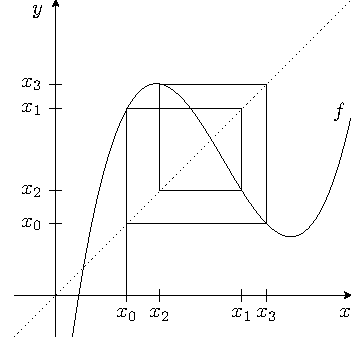
\includegraphics[]{images/iteracije_f.pdf}
% \caption[caption za v kazalo]{Dolg caption pod sliko}
  \caption[Primer vektorske slike.]{Slika prikazuje, iteracije funkcije $f$.}
  \label{fig:iteracije}
\end{figure}

V takem dinamičnem sistemu ena iteracija funkcije predstavlja en diskreten korak v času, točka $x_0 \in I$ pa začetni položaj točke v sistemu. Množici, ki vsebuje vse člene zaporedja $\left( x_n \right)_{n=0}^{\infty}$ bomo rekli \emph{$f$-orbita točke $x_0$} ali samo orbita točke $x_0$. Z matematičnimi simboli jo lahko zapišemo tako:
$$\{ \mathcal{O} := f^m(x_0) ; m \in \N \}.$$
Izrek Šarkovskega preučuje take točke $x_0 \in I$, ki se po nekaj iteracijah s funkcijo $f$ slikajo nazaj vase. Takim točkam rečemo \emph{periodične točke}. \emph{Perioda točke} $x_0$ je najmanjše tako naravno število $m$, za katero je $f^m(x_0) = x_0$. Ekvivalentno lahko sklepamo, da je orbita periodične točke $x_0$ končna množica, število različnih elementov v orbiti pa je enako periodi točke $x_0$. \emph{Negibna točka} (včasih ji rečemo tudi fiksna točka) je periodična točka s periodo 1, torej taka točka $x_0$, za katero je $f(x_0) = x_0$. Če obstaja periodična točka s periodo $n$, rečemo tudi, da ima funkcija $f$ periodo $n$.

Pri danem dinamičnem sistemu se lahko vprašamo, katere periode lahko ima funkcija. Šarkovski si je postavil prav to vprašanje in prišel do ureditve množice naravnih števil, ki pove, katere periode lahko ima funkcija.

\subsection{Izrek Šarkovskega}

\begin{definicija}
Množico naravnih števil lahko uredimo na naslednji način:
$$3 \triangleleft 5 \triangleleft 7 \triangleleft \cdots \triangleleft 2\cdot 3 \triangleleft 2\cdot 5 \triangleleft 2\cdot 7 \triangleleft \cdots \triangleleft 2^2\cdot 3 \triangleleft 2^2\cdot 5 \triangleleft 2^2\cdot 7 \triangleleft \cdots \triangleleft 2^3 \triangleleft 2^2 \triangleleft 2 \triangleleft 1.$$
Ureditev, imenujemo jo ureditev Šarkovskega, določa relacijo $\triangleleft$. Naravni števili $m$ in $n$ sta v relaciji $m\triangleleft n$ natanko tedaj, ko $m$ leži levo od $n$ ali je $m=n$. Opazimo, da je ureditev sestavljena tako, da najprej po vrsti naštejemo liha števila večja od 1, nato dodamo ta števila po vrsti pomnožena z 2. Sledijo liha števila večja od 1 pomnožena z $2^2$ itn. Na koncu so zapisane potence števila 2 v padajočem vrstnem redu. Zaradi vrstnega reda števil pomislimo, da lahko vsako naravno število zapišemo kot produkt potence števila 2 in nekega lihega števila. To pomeni, da lahko poljubni naravni števili $m$ in $n$ zapišemo na naslednji način: 
\begin{equation}
m= 2^k(2m_1 +1)\text{ in } n= 2^l(2n_1 +1), \label{eq:zapis}
\end{equation}
 kjer so števila $m_1, n_1, k, l \in \N_0$. Števili sta v relaciji $m \triangleleft n$, če je:
\begin{enumerate}[label={(R\arabic*)}]
\item $k<l$ in $m_1 \neq 0$ in $n_1 \neq 0$ ali \label{rel1}
\item $k=l$ in $0<m_1 \leq n_1$ ali \label{rel2}
\item $k \geq l$ in $m_1 = n_1=0$ ali \label{rel3}
\item $m_1>0$ in $n_1 =0$. \label{rel4}
\end{enumerate}
\end{definicija}

\begin{trditev}
Relacija $\triangleleft$, ki smo jo definirali, je relacija linearne urejenosti.
\end{trditev}
\begin{proof}
Za dokaz potrebujemo tri poljubna naravna števila:
\begin{itemize}
\item $m= 2^k(2m_1 +1)$,
\item $n= 2^l(2n_1 +1)$ in
\item $s=2^h(2s_1+1$.
\end{itemize}
Dokazati moramo refleksivnost, antisimetričnost, tranzitivnost in sovisnost relacije.
Refleksivnost: če je število $m$ liho, točka~\ref{rel3} zagotavlja, da je $m \triangleleft m$. Če je število $m$ sodo, pa relacija $m \triangleleft m$ sledi iz točke~\ref{rel2}.

Antisimetričnost: denimo, da za števili $m$ in $n$vveljata relaciji $m \triangleleft n$ in $n \triangleleft m$. Pogoja~\ref{rel1} in~\ref{rel4} za relacijo $m \triangleleft n$ sta v protislovju z vsemi pogoji relacije $n \triangleleft m$. Edina možnost, ki zadosti vsem potrebnim pogojem relacij je $k=l$ in $m_1 = n_1$. Torej je $m=n$.

Tranzitivnost: obravnavamo števila $m$,  $n$ in $s$, ki zadoščajo relacijam $m \triangleleft n$ in $n \triangleleft s$. Radi bi videli sta števili $m$ in $s$ v relaciji $m \triangleleft s$. Ker imamo 4 pogoje za relacijo $m \triangleleft n$ in 4 pogoje za relacijo $n \triangleleft s$, moramo obravnavati 16 možnih kombinacij. Vse kombinacije pogojev za relacije so zapisane v tabeli~\ref{table:1}. V drugem stolšcu so zapisani pogoji, ki jih dobimo iz relacije $m \triangleleft n$, v tretjem stoplcu so pogoji, ki jih preberemo iz relacije $n \triangleleft s$. V četrti stolpec smo zapisali pogoj, ki sledi iz pogojev v drugem in tretjem stolpcu. Opazimo, da v devetih primerih pogoja ne moreta biti izpolnjena istočasno, zato pridemo do protislovja. V ostalih primerih, pa dobimo enega od pogojev za relacijo $m \triangleleft s$, zato sta števili $m$ in $s$ v relaciji $m \triangleleft s$.

\begin{table}[h!]
\centering
\begin{tabular}{||c | l | l | l||} 
 \hline
 Col1 & $m \triangleleft n$ & $n \triangleleft s$ & $\Rightarrow$ \\ [0.5ex] 
 \hline\hline
 1 & $k<l$ in $m_1, n_1 \neq 0$ & $l<h$ in $n_1, s_1 \neq 0$ & $k<h$ in $m_1, s_1 \neq 0$ \\ 
 2 & $k<l$ in $m_1, n_1 \neq 0$ & $l=h$ in $0<n_1 \leq s_1$ & $k<h$ in $m_1, s_1 \neq 0$ \\
 3 & $k<l$ in $m_1, n_1 \neq 0$ & $l \geq h$ in $n_1 = s_1 = 0$ & protislovje \\
 4 & $k<l$ in $m_1, n_1 \neq 0$ & $n_1 = 0$, $s_1 > 0$ & $m_1 = 0$, $s_1 > 0$ \\
 5 & $k=l$ in $0<m_1 \leq n_1$ & $l<h$ in $n_1, s_1 \neq 0$ & protislovje \\ 
 6 & $k=l$ in $0<m_1 \leq n_1$ & $l=h$ in $0<n_1, s_1$ & $k=h$ in $0<m_1 \leq s_1$ \\
 7 & $k=l$ in $0<m_1 \leq n_1$ & $l \geq h$ in $n_1 = s_1 = 0$ & protislovje \\
 8 & $k=l$ in $0<m_1 \leq n_1$ & $k<l$ in $n_1 = 0$, $s_1 > 0$ & $m_1 = 0$, $s_1 > 0$ \\
 9 & $k \geq l$ in $m_1 = n_1 = 0$ & $l<h$ in $n_1, s_1 \neq 0$ & protislovje \\ 
 10 & $k \geq l$ in $m_1 = n_1 = 0$ & $l=h$ in $0<n_1, s_1$ & protislovje \\
 11 & $k \geq l$ in $m_1 = n_1 = 0$ & $l \geq h$ in $n_1 = s_1 = 0$ & $k \geq h$ in $m_1 = s_1 = 0$ \\
 12 & $k \geq l$ in $m_1 = n_1 = 0$ & $k<l$ in $n_1 = 0$, $s_1 > 0$ & protislovje \\
 12 & $m_1 = 0$, $n_1 > 0$ & $l<h$ in $n_1, s_1 \neq 0$ & protislovje \\ 
 14 & $m_1 = 0$, $n_1 > 0$ & $l=h$ in $0<n_1, s_1$ & protislovje \\
 15 & $m_1 = 0$, $n_1 > 0$ & $l \geq h$ in $n_1 = s_1 = 0$ & $m_1 = 0$, $s_1 > 0$ \\
 16 & $m_1 = 0$, $n_1 > 0$ & $k<l$ in $n_1 = 0$, $s_1 > 0$ & protislovje \\[1ex] 
 \hline
\end{tabular}
\caption{Vseh 16 možnosti.}
\label{table:1}
\end{table}

Sovisnost: prepričati se moramo, da za vsaki dve naravni števili $m, n$ velja $m \triangleleft n$ ali $n \triangleleft m$. Torej velja en od pogojev:
\begin{enumerate}[label={(\roman*)}]
\item $k<l$ in $m_1 \neq 0$ in $n_1 \neq 0$ ali \label{sov1}
\item $k=l$ in $0<m_1 \leq n_1$ ali \label{sov2}
\item $k \geq l$ in $m_1 = n_1=0$ ali \label{sov3}
\item $m_1>0$ in $n_1 =0$. \label{sov4}
\end{enumerate}
ali 
\begin{enumerate}[label={(\roman*)}]
\setcounter{enumi}{4}
\item $l<k$ in $m_1 \neq 0$ in $n_1 \neq 0$ ali \label{sov5}
\item $l=k$ in $0<n_1 \leq m_1$ ali \label{sov6}
\item $l \geq k$ in $m_1 = n_1=0$ ali \label{sov7}
\item $n_1>0$ in $m_1 =0$. \label{sov8}
\end{enumerate}
Denimo, da števili $m$ in $n$ nista v relaciji. Iz~\ref{sov4} in~\ref{sov8} ugotovimo, da mora biti $m_1 = n_1 = 0$ ali $m_1, n_1 \neq 0$. Ker števili ne ustrezata pogoju~\ref{sov3} niti pogoju~\ref{sov7} ugotovimo, da morata biti števili $m_1$ in $n_1$ različni od 0. Iz pogojev~\ref{sov1} in~\ref{sov5} sklepamo, da mora biti $k=l$. Sedaj pa števili zagotovo zadoščata enemu od pogojev~\ref{sov2} ali~\ref{sov6}. To je preotislovje s predpostavko, da števili $m$ in $n$ nista v relaciji. Torej res za vsaki dve naravni števili $m, n$ velja relacija $m \triangleleft n$ ali relacija $n \triangleleft m$. 
\end{proof}

Relacija $\triangleleft$ ima še eno zanimivo in za dokaz izreka Šarkovskega zelo pomembno lastnost.
\begin{trditev}
Števili $m$ in $n$ sta v relaciji $m \triangleleft n$ natanko tedaj, ko sta velja relacija $2m \triangleleft 2n$. Zapisano z matematičnimi simboli:
$$\text{za } \forall m, n \in \N: m \triangleleft n \Leftrightarrow 2m \triangleleft 2n.$$
\end{trditev}
\begin{dokaz}
Zapišimo števili $m$ in $n$ kot produkt potence števila 2 in nekega lihega števila:
$$m= 2^k(2m_1 +1)\text{ in } n= 2^l(2n_1 +1).$$
Če števili pomnožimo z 2, dobimo:
$$m= 2^{k+1}(2m_1 +1)\text{ in } n= 2^{l+1}(2n_1 +1).$$
Sedaj lahko preverimo, da so pogoji za relacijo $m \triangleleft n$ in relacijo $2m \triangleleft 2n$ ekvivalentni. To je očitno takoj, ko opazimo, da se števili $m_1$ in $n_1$ nista spremenili. Neenačbi $k<l$ in $k+1<l+1$ pa sta ekvivalentni. Podobno ugotovimo za neenačbi $k \geq l$ in $k+1 \geq l+1$ in enačbi $k=l$ in $k+1 = l+1$.
\end{dokaz}

Sedaj smo definirali vse potrebne pojme in spoznali tudi ureditev Šarkovskega. Čas je, da si poglejdamo na kakšen način ureditev Šarkovskega določa periode funkcije.

\begin{izrek}[The Sharkovsky forcing theorem]\label{izr:forcing}
Če ima $f : I \to I$ točko periode $m$ in velja $ m \triangleleft l$, potem obstaja tudi točka periode $l$.
\end{izrek}
Izrek pove, da je množica period zvezne funkcije na intervalu $I$ rep ureditve Šarkovskega. Rep ureditve Šarkovskega je taka množica $\mathcal{T} \subset \N$, za katero je $m \triangleleft n$ za  vsaki naravni števili $m \notin \mathcal{T}$ in $n \in \mathcal{T}$. Obstajajo trije različni tipi repov:  Za neko naravno število $m$ je rep množica $\{n \in \N; m \triangleleft n\}$, množica $\{\dots, 16, 8, 4, 2, 1\}$ vseh potenc števila 2 in $\emptyset$.
Naslednji izrek je neke vrste obrat zgornjega izreka.

\begin{izrek}[The Sharkovsky realization theorem]\label{izr:realization}
Za vsak rep $\mathcal{T}$ v zaporedju Šarkovskega obstaja taka funkcija $f$, katere množica period je enaka $\mathcal{T}$.
\end{izrek}

Izrek Šarkovskega je unija izreka~\ref{izr:forcing} in izreka~\ref{izr:realization}. Podmnožica naravnih števil je množica period zvezne funkcije $f:I \to I$, če in samo če je množica rep ureditve Šarkovskega. Nasledja poglavja so namenjena pripravi na dokaz izreka~\ref{izr:forcing}, v poglavju~\ref{sec:realizacija} pa je predstavljen dokaz izreka~\ref{izr:realization}.
\section{Intervali, relacija pokritja in cikli}
Vsi dokazi izreka Šarkovskega so si podobni po tem, da so elementarni. Ne glede na to, kako zvito se lotimo dokaza, je ključnega pomena lastnost zveznih funkcij, ki ob določenih predpostavkah zagotavlja obstoj ničle funkcije. To je izrek o vmesni vrednosti.

\begin{izrek}[izrek o vmesni vrednosti]\label{izr:iovv}
Funkcija $f$, ki je zvezna na intervalu $[a, b]$ in je na krajiščih intervala različno predznačena, torej velja neenačba $f(a)\cdot f(b) < 0$, ima vsaj v eni točki tega intervala vrednost 0.
\end{izrek}

\begin{figure}[h]
  \centering
  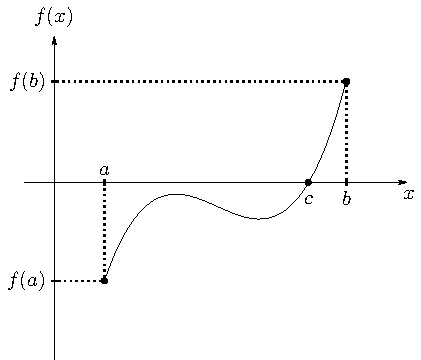
\includegraphics[]{images/intermediate.pdf}
% \caption[caption za v kazalo]{Dolg caption pod sliko}
  \caption[Primer vektorske slike.]{Slika prikazuje, kako poiščemo interval $K$.}
  \label{fig:bezje}
\end{figure}

\begin{proof}
Naj bo funkcija $f:[a, b] \to [a, b]$ zvezna in naj bo $f(a)\cdot f(b) < 0$. Brez izgube splošnosti lahko predpostavimo, da je $f(a) < 0 < f(b)$. Ničlo funkcije $f$ bomo iskali s pomočjo deljenja intervalov oziroma z bisekcijo. Izračunamo razpolovišče $p_0=\frac{a+b}{2}$ intervala $[a, b]$.Če je $f(p_0)=0$, smo ničlo že našli, sicer razmišljamo tako: če je $f(p_0) >0$, označimo $[a_1, b_1] =  [a, p_0]$, sicer označimo $[a_1, b_1] =  [p_0, b]$. Nato izračunamo razpolovišče $p_1$ intervala $[a_1, b_1]$. Če je $f(p_1)=0$ postopek ustavimo, saj smo ničlo našlio, v nasprotnem primeru pogledamo predznak $f(p_1)$. Če je $f(p_1) >0$, označimo $[a_2, b_2] =  [a_1, p_1]$, drugače označimo $[a_2, b_2] =  [p_1, b_1]$. Postopek nadaljujemo dokler ne najdemo ničle $p_i$ funkcije $f$. Če ničle ne najdemo, dobimo neskončno zaporedje vloženih intervalov 
$$ [a, b] \supset [a_1, b_1] \supset [a_2, b_2] \supset \cdots$$
Lahko se prepričamo, da je $b_n - a_n = \frac{b-a}{2^n}$ in $f(a_n)<0<f(b_n)$ za vsak $n\in \N$. Števila $a_n$ tvorijo naraščajoče zaporedje, števila $b_n$ pa padajoče zaporedje.  Limiti $\lim\limits_{n \to \infty} a_n$ in $\lim\limits_{n \to \infty} b_n$ sta enaki, saj je 
$\lim\limits_{n \to \infty} b_n - \lim\limits_{n \to \infty} a_n = \lim\limits_{n \to \infty} (b_n - a_n) =0$. Označimo $c = \lim\limits_{n \to \infty} a_n = \lim\limits_{n \to \infty} b_n$. Točka $c$ je večja od vseh členov zaporedja $\left(a_n \right)_{n=1}^{\infty}$ in manjša od vseh členov zaporedja $\left(b_n \right)_{n=1}^{\infty}$, zato je za vsak $n \in \N$ vsebovana v intervalu $[a_n, b_n]$. Torej velja:
$\bigcap\limits_{n=1}^{\infty} [a_n, b_n] = \{c\}$. 
Ker je funkcija zvezna je 
$\lim\limits_{n \to \infty} f(a_n) = f(\lim\limits_{n \to \infty} a_n) = f(c)$
in 
$\lim\limits_{n \to \infty} f(b_n) = f(\lim\limits_{n \to \infty} b_n) = f(c)$.
Za vsako naravno število $n$ velja $f(a_n) <0$, zato je $f(c) \leq 0$. Podobn je $f(b_n) > 0$ za vsako naravno število $n$, iz česar sklepamo, da je $f(c) \geq 0$. Torej je $f(c) = 0$, kar zaključi dokaz.
\end{proof}

\begin{definicija}\label{def:pokritja}
Pravimo, da interval $I$ pokrije interval $J$, če je $J \subseteq f(I)$. Relacijo zapišemo kot $I \xrightarrow{f} J$. Kadar je jasno, katera funkcija nastopa, lahko nadpis, ki označi katero funkcijo imamo v mislih tudi izpustimo in pišemo samo $I \to J$. Če velja $f(I) =J$, zapišemo $I \rightarrowtail J$.
\end{definicija}

S pomočjo izreka o vmesni vrednosti in poznavanja, kako se intervali slikajo s funkcijo $f$ lahko izvemo, ali obstajajo periodične točke. Kako lahko potrdimo obstoj periodičnih točk, nam povejo naslednje leme.

\begin{lema}\label{lem:1zanka}
Če je $[a, b] \to [a, b]$, potem ima funkcija $f$ fiksno točko na intervalu $[a, b]$.
\end{lema}
\begin{proof}
Interval $[a, b]$ je podmnožica slike $f([a, b])$, zato obstajata taki točki $a_1, b_1 \in [a, b]$, da je $f(a_1)=a$ in $f(b_1)=b$. Če je $a_1 = a$ ali $b_1 = b$, smo fiksno točko že našli. Če je $a_1 \neq a$ in $b_1 \neq b$, definiramo funkcijo $g(x) = f(x) - x$. Prepričajmo se, da je vrednost funkcije $g$ v točki $b_1$ negativna, v točki $a_1$ pa pozitivna. Računamo:
$g(b_1) = f(b_1) - b_1 = b - b_1 < 0$. Podobno je
$g(a_1) = f(a_1) - a_1 = a - a_1 > 0$.
Zvezna funkcija $g$ je na krajiščih intervala $[a, b]$ različno predznačena. Po izreku~\ref{izr:iovv} obstaja točka $c \in [a, b]$, pri kateri je $g(c)=0$, torej je $f(c) = c$.
\end{proof}
Pri iteracijah funkcije lahko opazujemo, kako se premika točka. To smo počeli na sliki~\ref{fig:iteracije}. Lahko pa opazujemo, kako se s $f$ slikajo celi intervali. Na ta način dobimo zaporedje relacij pokritja npr. $I_0 \to I_1 \to I_2 \to \cdots $. Enako kot pri periodičnih točkah lahko pri zaporedu relacij pokritja po nekaj korakih zopet pridemo do prvotnega intervala. Dobimo naslednje zaporedje relacij pokritja $I_0 \to I_1 \to \cdots \to I_n \to I_0$. Če je začetni interval enak končnemu intervalu, zaporedju intervalov in pripadajočim relacijam pokritja pravimo \emph{zanka intervalov} ali samo zanka. Od tu naprej bo interval predstavljal zaprto, omejeno in povezano podmnožico realnih števil.

\begin{lema}\label{lem:zanka}
Če so intervali $I_0, \dots, I_{n-1}$ intervali, za katere veljajo naslednje relacije pokritosti: $I_0 \to I_1 \to \dots \to I_{n-1} \to I_0$, potem obstaja taka točka $c \in I_0$, za katero je $f^{i}(x) \in I_i$ za $0 \leq i < n$ in $f^n(c)=c$. Pravimo, da točka $c$ sledi zanki.
\end{lema}

\begin{proof}
Če velja relacija pokritosti $I \to J$, obstaja tak interval $K \subset I$, da je $K \rightarrowtail J$.
\begin{figure}[h]
  \centering
  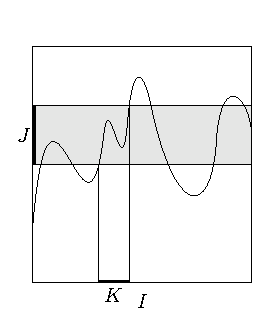
\includegraphics[]{images/bezje.pdf}
% \caption[caption za v kazalo]{Dolg caption pod sliko}
  \caption[Primer vektorske slike.]{Slika prikazuje, kako poiščemo interval $K$.}
  \label{fig:bezje}
\end{figure}
Interval $K$ poiščemo tako, da iz preseka funkcije $f$ s pravokotnikom $I \times J$ izberemo povezan del grafa, ki povezuje spodni in zgornji del pravokotnika. Tak del zagotovo obstaja, saj je $J \subset f(I)$. Projekcijo tega dela na interval $I$ označimo s $K$. To znanje uporabimo na zanki intervalov $I_0 \to \dots \to I_{n-1} \to I_0$. Ker velja relacija pokritja $I_{n-1} \to I_0$, vemo, da obstaja tak interval $K_{n-1} \subset I_{n-1}$, da je $K_{n-1} \rightarrowtail I_0$. Velja relacija pokritosti $I_{n-2} \to K_{n-1}$, zato obstaja tak interval $K_{n-2} \subset I_{n-2}$, da je $K_{n-2} \rightarrowtail K_{n-1}$. S postopkom nadaljujemo in dobimo naslednje relacije:
$$K_0 \rightarrowtail K_1 \rightarrowtail \cdots \rightarrowtail K_{n-1} \rightarrowtail I_0.$$
Za vsako točko $x \in K_0$ in za vsak $i \in [0, n)$ velja $f^i(x) \in K_i \subset I_i$ in $f^n(x) \in I_0$. Ker je $K_0 \subset I_0 = f^n(K_0)$, lahko s pomočjo leme~\ref{lem:1zanka} sklepamo, da ima $f^n$ fiksno točko $c$ na intervalu $K_0$. Točka $c$ sledi zanki $I_0 \to \dots \to I_{n-1} \to I_0$.
\end{proof}

Pri dokazovanju izreka bomo dokazali obstoj zank različnih dolžin. Želeli bi si, da je perioda točke, ki sledi zanki enaka dolžini zanke. 

\begin{definicija}\label{def:element}
Zanka intervalov $I_0 \to I_1 \to \cdots \to I_{n-1} \to I_0$ je elementarna, če ima vsaka točka, ki sledi zanki, periodo $n$.
\end{definicija}

\begin{posledica}
Vsaka elementarna zanka intervalov $I_0 \to I_1 \to \dots \to I_{n-1} \to I_0$ vsebuje točko $x_0$, ki sledi zanki in ima periodo $n$.
\end{posledica}

Zaradi zgornje posledice bi bilo dobro, če bi poznali kakšen dober kriterij za prepoznavanje elementarnih zank. Najlažji kriterij je število intervalov v zanki. Če nastopa samo en interval, dobimo zanko $I_0 \to I_0$. Z uporabo leme~\ref{lem:1zanka} ugotovimo, da je zanka elementarna. Naslednja lema pove, da sta  poda še en kriterij za prepoznavanje elementarnih zank:

\begin{lema}\label{lem:element}
Zanka intervalov $I_0 \to I_1 \to \cdots \to I_{n-1} \to I_0$ je elementarna, če ji ne sledi nobena robna točka intervala $I_0$ in je notranjost intervala $\interior(I_0)$ disjunktna z intervali $I_1, I_2,  \dots, I_{n-1}$. Torej, $\interior(I_0) \cap \bigcup_{i=1}^{n-1}I_i = \emptyset$.
\end{lema}
\begin{proof}
Točka $x_0$, ki sledi zanki ne more biti robna točka intervala $I_0$. Torej je $x_0 \in \interior(I_0)$. Za vsak $i=1, \dots, n-1$ je $x_0 \neq f^i(x_0)$, saj je $f^i(x_0) \in I_i$, notranjost intervala $I_0$ pa je disjunktna z intervalom $I_i$. Ker točka $x_0$ sledi zanki, je $f^n(x_0)=x_0$. Točka $x_0$ ima periodo $n$.
\end{proof}

Poglejmo si dva primera, ki pokažeta, da nobene predpostavke v lemi~\ref{lem:element} ne moremo izpustiti.

\begin{primer}
Obravnavajmo zvezno funkcijo $f(x) = -\sqrt[3]{x}$ in 2-zanko intervalov $[0, \frac{1}{2}] \leftrightarrows [-\frac{1}{2}, 0]$. Samo ena točka sledi tej zanki, to je točka 0. Perioda točke 0 ni enaka enaka dolžini zanke, saj je točka 0 negibna točka in je njena perioda enaka 1.
\end{primer}
\begin{primer}
Funkcija $f(x) = - x^2$ tvori $2$-zanko $[\frac{1}{4}, \frac{9}{4}] \leftrightarrows [\frac{1}{2}, 4]$. Tej zanki sledi zgolj točka $1$, ki je negibna točka, torej je njena perioda različna od dolžine zanke.
\end{primer}
Zanka v primeru 1 ni elementarna, saj ji sledi robna točka začetnega intervala. Zanka v primeru 2 pa ni elementarna, saj točka 1 leži v preseku notranjosti prvega intervala in drugega intervala. 

\begin{definicija}
Zaprt in omejen interval, katerega krajišči pripadata ciklu $\mathcal{O}$ imenujemo $\mathcal{O}$-interval. 
\end{definicija}
V nadaljevanju bomo zgornje leme uporabili na $\mathcal{O}$-intervalih. Tako bomo poenostavili obravnavo periodičnih točk funkcije $f$, saj bomo uporabili samo informacije, ki jih lahko pridobimo iz delovanja funkcije $f$ na ciklu $\mathcal{O}$. Zato bodo naši sklepi veljali za vse zvezne funkcije s ciklom $\mathcal{O}$. Relaciji pokritja $I \to J$ rečemo $\mathcal{O}$-vsiljena, če interval $J$ leži v $\mathcal{O}$-intervalu $M$ katerega krajišči sta skrajno leva in skrajno desna točka množice $f(I \cap \mathcal{O})$. Ker je funkcija $f$ zvezna, lahko s pomočjo izreka~\ref{izr:iovv} ugotovimo, da je množica $f(I)$ interval. Velja $J \subset M \subset f(I)$. V nadaljevanju dela bodo vse relacije pokritja $\mathcal{O}$-vsiljene. Zanka intervalov $I_0 \to I_1 \to \cdots \to I_{n-1} \to I_0$, v kateri vsaka puščica predstavlja $\mathcal{O}$-vsiljeno relacijo pokritja, se imenuje $\mathcal{O}$-vsiljena zanka $\mathcal{O}$-intervalov.

Vse relacije pokritja, o katerih bomo govorili, bodo $\mathcal{O}$-vsiljene, zato bodo vse relacije pokritja, ki jih bomo označili s simbolom `'$\to$'', predstavljale $\mathcal{O}$-vsiljene relacije pokritja.


\section{Primeri}%################ POGLAVJE S PRIMERI
V tem poglavju si bomo zaradi lažjega razumevanja pogledali nekaj posebnih primerov. Najprej si bomo pogledali najbolj znan poseben primer izreka Šarkovskega. V naslednjih dveh primerih bomo postopek iz prvega primera razširili na daljše cikle. V zadnjem primeru bomo nakazali kako lahko iz periodičnih točk funkcije $f^2$ ugotovimo katere periode ima funkcija $f$, kar igra pomembno vlogo pri dokazu izreka~\ref{izr:forcing}.

\begin{primer}[3-cikel]\label{primer1}
Perioda 3 implicira obstoj vseh ostalih period. Točka lahko tvori $3$-cikel na dva različna načina, ki sta v resnici zrcalna podoba drug drugega. Slika prikazuje oba primera. 
\begin{figure}[h]
  \centering
  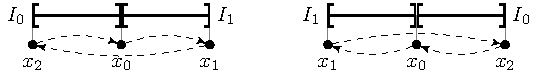
\includegraphics{images/tricikel.pdf}
% \caption[caption za v kazalo]{Dolg caption pod sliko}
  \caption[Primer vektorske slike.]{Zrcalna podoba ciklov}
  \label{fig:3cikla}
\end{figure}
Črtkane puščice nakazujejo, kam se s funkcijo $f$ slikajo točke. Velja: 
$$x_1 = f(x_0), x_2 = f(x_1) \text{ in } x_0 = f(x_2).$$
V obeh primerih smo z $I_1$ označili $\mathcal{O}$-interval s krajišči $x_0$ in $x_1$, z $I_0$ pa $\mathcal{O}$-interval s krajišči $x_0$ in $x_2$. Krajišči intervala $I_1$ se slikata v skrajno levo in skrajno desno točko cikla, zato imamo $\mathcal{O}$-vsiljeni pokritji $I_1 \to I_1$ in $I_1 \to I_0$. Krajišči intervala $I_0$ se slikata v krajišči intervala $I_1$, zato je tudi pokritje $I_0 \to I_1$ $\mathcal{O}$-vsiljeno. Ugotovljena pokritja lahko strnemo v diagram $\sara I_1 \leftrightarrows I_0$. Iz relacije pokritosti $I_1 \to I_1$ in leme~\ref{lem:1zanka} sklepamo, da interval $I_1$ vsebuje negibno točko. Krajišči intervala $I_0$ ne morejo slediti zanki $I_0 \to I_1 \to I_0$, saj sta periodični točki s periodo 3. Točke, ki sledijo zanki, pa imajo periodo 1 ali 2. Ker je notranjost intervala $I_0$ disjunktna z intervalom $I_1$, lahko s pomočjo leme~\ref{lem:element} sklepamo, da je zanka elementarna. Torej lahko v intervalu $I_0$ poiščemo točko s periodo 2. Za dokaz obstoja točke s periodo $l\geq 4$ si poglejmo zanko
\begin{equation}
I_0 \to \overbrace{I_1 \to I_1 \to \cdots \to I_1}^{l-1 \text{ ponovitev intervala } I_0} \to I_0. \label{eq:lzanka}
\end{equation}
V tej zanki nastopajo vsaj 3 kopije intervala $I_1$, v katerem ležita samo dve točki $\mathcal{O}$-intervala. Ker imajo točke iz cikla $\mathcal{O}$ periodo 3, v intervalu $I_1$ ne morejo ležati trije zaporedni členi iz cikla $\mathcal{O}$, torej tudi tri zaporedne iteracije funkcije $f$ na krajiščih intervala $I_0$ ne morejo ležati v intervalu $I_1$. To pomeni, da krajišči intervala $I_0$ ne moreta slediti zanki. Že prej smo ugotovili, da je notranjost intervala $I_0$ disjunktna z intervalom $I_1$, zato je zanka~\eqref{eq:lzanka} elementarna zanka dolžine $l$. Zato ima funkcija $f$ periodo $l$ za vsak $l \geq 4$. Pokazali smo, da je vsako naravno število perioda funkcije $f$.
\end{primer}


\begin{primer}[7-cikel] \label{primer2}
Sedaj bomo obravnavali 7-cikel $\mathcal{O}$ in $\mathcal{O}$-intervale prikazane na sliki~\ref{fig:7cikel}.
\begin{figure}[h]
  \centering
  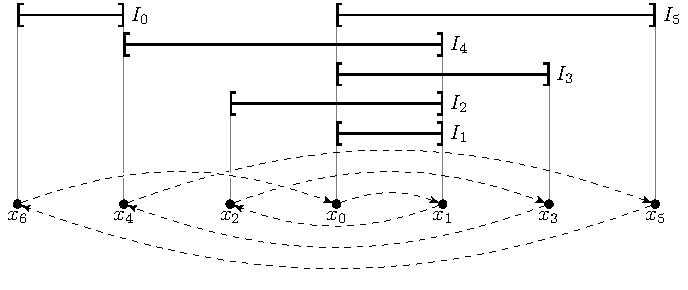
\includegraphics{images/sedemcikel.pdf}
% \caption[caption za v kazalo]{Dolg caption pod sliko}
  \caption[Primer vektorske slike.]{Primer 7-cikla.}
  \label{fig:7cikel}
\end{figure}
 Podobno kot pri prejšnjem primeru označimo točke $x_i = f^i(x_0)$ ter intervale $I_1 = [x_0, x_1]$, $I_2 = [x_1, x_2]$  in tako naprej kot prikazuje slika~\ref{fig:7cikel}. Za to izbiro intervalov dobimo naslednje $\mathcal{O}$-vsiljene relacije pokritosti:
\begin{enumerate}
\item $I_1 \to I_1$
\item $I_1 \to I_2 \to I_3 \to I_4 \to I_5 \to I_0$
\item $I_0 \to I_1$, $I_0 \to I_3$ in $I_0 \to I_5$
\end{enumerate}
Zgornje relacije pokritosti lahko prikažemo z diagramom, ki ga prikazuje slika~\ref{fig:6kotnik}.
\begin{figure}[h]
  \centering
  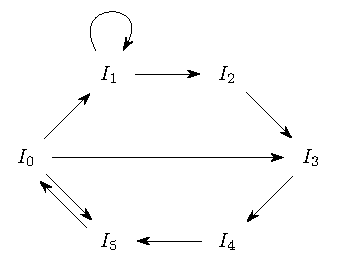
\includegraphics{images/graph6.pdf}
% \caption[caption za v kazalo]{Dolg caption pod sliko}
  \caption[Primer vektorske slike.]{diagram}
  \label{fig:6kotnik}
\end{figure}
Iz grafa preberemo naslednje zanke.
\begin{enumerate}
\item $I_1 \to I_1$
\item $I_0 \to I_5 \to I_1$ \label{7cikelz2}
\item $I_0 \to I_3 \to I_4 \to I_5 \to I_0$ \label{7cikelz3}
\item $I_0 \to I_1 \to I_2 \to I_3 \to I_4 \to I_5 \to I_0$ \label{7cikelz4}
\item $I_0 \to \underbrace{I_1 \to I_1 \to \cdots  \to I_1}_{l \text{ ponovitev intervala } I_1} \to I_2 \to I_3 \to I_4 \to I_5 \to I_0$, kjer je $l\geq 3$. \label{7cikelz5}
\end{enumerate}
Zanka $I_1 \to I_1$ je elementarna, saj je elementarna vsaka zanka dolžine 1. Pri ostalih zankah lahko najprej ugotovimo, da za vsak $j \in \{1, 2, \dots, 5\}$ velja $\interior(I_0) \cap I_j = \emptyset$. Pri zankah~\ref{7cikelz2},~\ref{7cikelz3} in~\ref{7cikelz4} nobena robna točka intervala $I_0$ ne more slediti zanki, saj je perioda robnih točk 7, perioda točk, ki sledijo zankam~\ref{7cikelz2},~\ref{7cikelz3} in~\ref{7cikelz4} pa je manjša ali enaka 6. Podobno kot v primeru~\ref{primer1} ugotovimo, da nobene tri zaporedne iteracije funkcije $f$ na točkah cikla $\mathcal{O}$ ne ležijo v intervalu $I_1$, zato v tem intervalu tudi ne morejo ležati tri zaporedne iteracije funkcije $f$ na robnih točkah intervala $I_0$. To pomeni, da krajišči intervala $I_0$ ne sledita zanki~\ref{7cikelz5}. S tem razmislekom so izpolnjeni pogoji leme~\ref{lem:element}, zato lahko sklepamo, da so zanke elementarne. Torej lahko na podlagi prisotnosti 7-cikla na sliki~\ref{fig:7cikel} sklepamo, da so prisotne vse periode $l$, za katere je $l \triangleleft 7$
\end{primer}

\begin{primer}[9-cikel] \label{primer3}
Predpostavimo, da ima funkcija $f$ 9-cikel $\mathcal{O}$, ki je prikazan na sliki~\ref{fig:9cikel}. 
\begin{figure}[h]
  \centering
  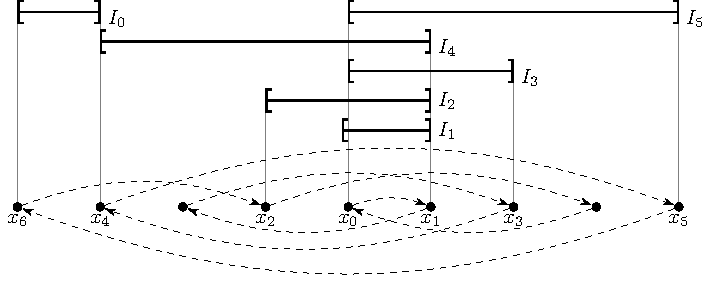
\includegraphics{images/devetcikel.pdf}
% \caption[caption za v kazalo]{Dolg caption pod sliko}
  \caption[Primer vektorske slike.]{Primer 9-cikla.}
  \label{fig:9cikel}
\end{figure}
Opazimo lahko, da smo določili šest $\mathcal{O}$-intervalov $I_0, I_1, \dots, I_5$, za katere velja, da je notranjost intervala $I_0$ disjunktna z ostalimi intervali. Torej za $j=1, 2, \dots, 5$ velja: $\interior{(I_0)} \cap I_j \neq \emptyset$. Za tako izbrane intervale dobimo enake relacije pokritja kot v primeru~\ref{primer1} in lahko s pomočjo enakih sklepov ugotovimo prisotnost enakih elementarnih zank in posledično periodičnih točk s periodami 1, 2, 4, 6 in vse periode večje od 7.

Zaporedje števil $x_0, x_1, \dots, x_6$ smo določili tako, da se spiralno oddaljujejo od centra $c:=\frac{x_0+x_1}{2}$, kar je prikazano na sliki~\ref{fig:spiral}. S tako izbiro točk pa v zaporedju ne nastopajo vse točke cikla $\mathcal{O}$ in tudi ne velja enakost $f(x_i) = x_{i+1}$ za vsak $i = 1, 2, \dots, 5$ kot je to veljalo v primeru~\ref{primer2}
\begin{figure}[h]
  \centering
  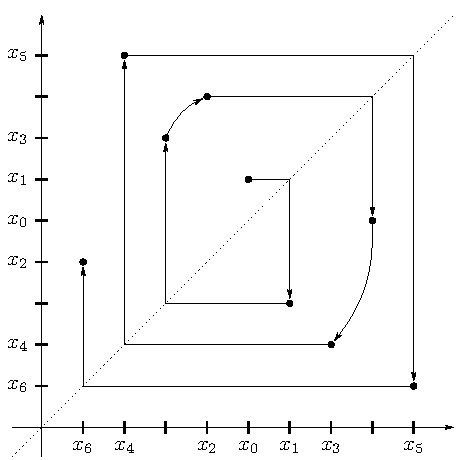
\includegraphics{images/spiral.pdf}
% \caption[caption za v kazalo]{Dolg caption pod sliko}
  \caption[Primer vektorske slike.]{Primer 9-cikla.}
  \label{fig:spiral}
\end{figure}

V poglavju~\ref{konssz} je predstavljen algoritem za izbiro zaporedja točk $x_0, x_1, \dots, x_6$. Glavna ideja algoritma je, da za naslednji člen zaporedja ne izberemo vedno sliko prejšnjega člena na način: $x_{i+1} = f(x_i)$, vendar včasih izberemo točko, ki je bližje centru $c$. Točko $x_{i+1}$, ki je bližje centra $c$ kot točka $f(x_i)$ izberemo, če je slika $f(x_{i+1})$ bolj oddaljena od centra kot točka $f(f(x_i))$. Postopka izbire naslednje točke na sliki~\ref{fig:iteracije} in na sliki~\ref{fig:spiral} sta podobna. V obeh primerih se pomikamo navpično do grafa funkcije in nato vodoravno do simetrale lihih kvadrantov. Sprememba se zgodi na sliki~\ref{fig:spiral}, ko lahko izberemo še neizbrano točko tako, da se v vodoravni smeri pomaknemo proti centru $c$, v navpični smeri pa stran od centra $c$. To se na sliki~\ref{fig:spiral} zgodi dvakrat in je prikazano s krivimi puščicami. 
Postopek se ustavi, ko pridemo do točke $x_j$, katere slika $f(x_j)$ je na isti strani centra $c$ kot točka sama. V primeru na sliki~\ref{fig:spiral} je to točka $x_6$.

V poglavju~\ref{stefan_zap} si bomo natančno pogledali kakšne lastnosti mora imeti zaporedje točk $x_0, x_1, \dots, x_{n-1}$, ki predstavlja krajišča intervalov $I_0, I_1, \dots, I_{n-1}$.

\end{primer}

\begin{primer}[6-cikel] \label{primer4}
Obravnavali bomo 6-cikel, ki je na sliki~\ref{fig:6cikel}. Bistveno pri tem primeu je, da se tri točke na levi strani slikajo v tri točke na desni in obratno. Torej, tri točke na desni tvorijo 3-cikel
\tikz{
\tikzset{vertex/.style = {shape=circle, fill=black,draw,minimum size=3pt, inner sep=0pt}}
\tikzset{edge/.style = {->,> = latex'}}
	\node [vertex](1) at  (0, 0) {};
	\node[vertex] (2) at  (0.8, 0) {};
	\node[vertex] (3) at  (1.6, 0) {};
	\draw[edge, dashed] (1) to[bend left=20] (2);
	\draw[edge, dashed] (2) to[bend left=20] (3);
	\draw[edge, dashed] (3) to[bend left=15] (1);
}
 za funkcijo $f^2$. Podobno kot v primeru~\ref{primer1} lahko določimo intervala $I_0$ in $I_1$ ter opazujemo relacije pokritja $I_1 \xrightarrow{f^2} I_1$, $I_1 \xrightarrow{f^2} I_0$ in $I_0 \xrightarrow{f^2} I_1$ za intervala $I_0$ in $I_1$, ki sta prikazana na sliki~\ref{fig:6cikel}. Enako kot prej lahko zaključimo, da ima funkcije $f^2$ elementarne zanke vseh dolžin in zato je vsako naravno število $l \in N$ perioda funkcije $f^2$. Za funkcijo $f$ določimo še dva intervala. Interval $I_0'$ naj bo najkrajši $\mathcal{O}$-interval, ki vsebuje točke iz množice $f(I_0 \cup \mathcal{O})$, interval $I_1'$ pa naj bo najkrajši $\mathcal{O}$-interval, ki vsebuje točke iz množice $f(I_1 \cup \mathcal{O})$. Sedaj bomo prikazali rekurzivno metodo, ki jo bomo uporabili kasneje v dokazu. Pokazali bomo, kako lahko s pomočjo elementarne $k$-zanke za funkcijo $f^2$ poiščemo elementarno $2k$-zanko za funkcijo $f$. V primeru, ki ga obravnavamo, bo to pomenilo, da je vsako sodo naravno število perioda funkcije $f$.
Poglejmo si elementarno $k$-zanko za funkcijo $f^2$, v kateri nastopajo relacije pokritja 
$I_1 \xrightarrow{f^2} I_1$, $I_1 \xrightarrow{f^2} I_0$ in $I_0 \xrightarrow{f^2} I_1$. Vsak zapis $I_1 \xrightarrow{f^2}$ v zanki lahko zamenjamo z $I_1 \xrightarrow{f} I_1'  \xrightarrow{f}$, vsak zapis $I_0 \xrightarrow{f^2} $ pa z $I_0 \xrightarrow{f} I_0'  \xrightarrow{f}$. S to spremembo dobimo $2k$-zanko za funkcijo $f$, ki ni samo dvakrat ponovljena $k$-zanka. Prepričajmo se, da je $2k$-zanka elementarna. Denimo, da točka $p$ sledi $2k$-zanki za funkcijo $f$. Pokazati moramo, da ima periodo $2k$ za funkcijo $f$. Opazimo, da točka $p$ sledi prvotni $k$-zanki za funkcijo $f^2$ in ima zato periodo $k$ za funkcijo $f^2$. Po drugi strani pa iteracije točke $p$ s funkcijo $f$ ležijo alternirajoče enkrat na levi in enkrat na desni strani srednjega intervala, saj $2k$-zanka za $f$ alternira med intervali s črtico in intervali brez črtice. Zato je orbita točke $p$ sestavljena iz $2k$ različnih točk. Na desni strani srednjega intervala leži $k$ sodih iteracij, na levi strani pa leži $k$ lihih iteracij. To pomeni, da ja perioda točke $p$ za $f$ enaka $2k$. Ker smo dolžino začetne elementarne $k$-zanke izbrali poljubno, smo pokazali, da je vsako sodo število perioda za $f$. Ker interval $[x_0, x_1]$ s funkcijo $f$ pokrije samega sebe, pa obstaja fiksna točka. Torej ima $f$ tudi periodo 1. 

\begin{figure}[h]
  \centering
  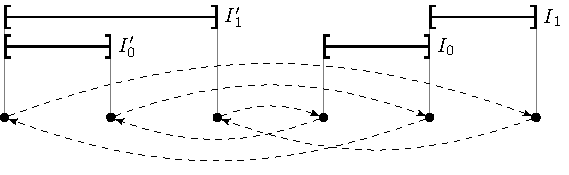
\includegraphics{images/sestcikel.pdf}
% \caption[caption za v kazalo]{Dolg caption pod sliko}
  \caption[Primer vektorske slike.]{Primer 6-cikla.}
  \label{fig:6cikel}
\end{figure}
\end{primer}

\section{Štefanovo zaporedje} \label{stefan_zap} 
V tem poglavju podamo definicijo Štefanovega zaporedja točk. Pokažemo, da te točke določajo intervale, s pomočjo katerih zapišemo relacije pokritja in ustrezne zanke, ki zagotavljajo obstoj periodičnih.
\begin{definicija}
Naj bo $p$ najbolj desna točka intervala $\mathcal{O}$, za katero je $f(p) > p$ in $q\in \mathcal{O}$ prva točka desno od p. Center $c$ cikla $\mathcal{O}$ definiramo kot $c=\frac{p+q}{2}$. Za vsako točko $x \in \mathcal{O}$ označimo množico točk iz cikla $\mathcal{O}$, ki ležijo v zaprtem intervalu omejenem z $x$ in $c$, z $\mathcal{O}_x$. Natančneje, $\mathcal{O}_x = \mathcal{O} \cap [x, p]$, če je $x \leq p$ in  $\mathcal{O}_x = \mathcal{O} \cap [q, x]$, če je $x \geq q$. Pravimo, da točka $x \in \mathcal{O}$ menja strani, če točka $c$ leži med točkama $x$ in $f(x)$.
\end{definicija}

\begin{definicija}
Zaporedje točk $x_0, x_1, \dots, x_n$ je Štefanovo, če:

  \begin{enumerate}[label={(Š\arabic*)}]
    \item $\{x_0, x_1\} = \{p, q\}$, \label{eq:š1}
    \item točke $x_1, x_2, \dots, x_n$ ležijo alternirajoče na levi oziroma desni strani točke $c$. \label{eq:š2}
    \item Zaporedji $x_{2j}$ in $x_{2j+1}$ sta strogo monotoni in se oddaljujeta od točke $c$. \label{eq:š3}
    \item Če je $1\leq j \leq n-1$, potem $x_j$ menja stran in $x_{j+1} \in \mathcal{O}_{f(x_j)}$.\label{eq:š4}
    \item Točka $x_n$ ne menja strani. \label{eq:š5}
  \end{enumerate}
  
\end{definicija}
\begin{opomba}
Štefanofo zaporedje dobimo tako, da iz množice $m$ točk, ki tvorijo $\mathcal{O}$-cikel izberemo $(n+1)$-o točko, ki zadoščajo zgornjim pogojem. 
Pogoj $x_{j+1} \in \mathcal{O}_{f(x_j)}$ v~\ref{eq:š4} pomeni, da je točka $x_{j+1}$ bližje centru kot slika $f(x_j)$ točke $x_j$. Velja ena od neenakosti: $c < x_{j+1} \leq f(x_j)$ ali $f(x_j) \leq x_{j+1} < c$. 
Pogoja~\ref{eq:š2} in~\ref{eq:š3} zagotavljata, da so točke $x_0, x_1, \dots, x_n$ paroma različne. Ker pa lahko pri izbiri točk iz $\mathcal{O}$-cikla tudi kakšno točko izpustimo, je število $n+1$ izbranih točk manjše ali enako številu vseh točk v $\mathcal{O}$-ciklu. Če se vrnemo na primere iz prejšnjega poglavja, lahko vidimo, da v primerih~\ref{primer1}, \ref{primer2} in \ref{primer4} Štefanovo zaporedje sestavljajo vse točke $\mathcal{O}$-cikla. V primeru~\ref{primer3} pa smo dve točki $\mathcal{O}$-cikla ne nastopata v Štefanovem zaporedju.
 Na slikiIz pogoja~\ref{eq:š2} lahko razberemo, da so točke $x_0, x_1, \dots, x_n$ paroma različne. Torej je $n+1 \leq m$ in zato $n<m$. Sliki~\ref{fig:7cikel}
\end{opomba}

\begin{trditev}\label{trd:zap-cikel}
Predpostavimo, da $m$-cikel $\mathcal{O}$ vsebuje Štefanovo zaporedje. Če je $l \triangleleft m$, potem funkcija $f$ vsebuje $\mathcal{O}$-vsiljeno elementarno $l$-zanko $\mathcal{O}$-intervalov in posledično tudi periodično točko z periodo $l$.
\end{trditev}

Pri danem Štefanovem zaporedju $x_0, x_1, \dots, x_n$ definiramo intervale $I_0, I_1, \dots, I_{n-1}$ na  nasledni način: Za $1 \leq j < n$, označimo z $I_j$ najkrajši $\mathcal{O}$-interval, ki vsebuje točke $x_0$, $x_1$ in $x_j$, medtem ko z $I_0$ označimo $\mathcal{O}$-interval s krajišči $x_{n-2}$ in $x_n$. Iz lastnosti~\ref{eq:š2} lahko sklepamo, da je $\interior(I_0) \cap I_j = \emptyset$ za vsak $j \in \{1, 2, \dots, n-1\}$.

\begin{trditev}\label{trd:pokritja}
Za intervale izbrane na zgoraj opisan način veljajo naslednje relacije pokritja:
\begin{enumerate}
\item $I_1 \to I_1$ in $I_0 \to I_1$,\label{trd:pokritja1}
\item $I_1 \to I_2 \to \cdots \to I_{n-1} \to I_0$,\label{trd:pokritja3}
\item $I_0 \to I_{n-1}, I_{n-3}, I_{n-5} \dots $.\label{trd:pokritja2}
\end{enumerate}
Zaradi boljše predstave ponazorimo relacije pokritja na sliki~\ref{fig:nkotnik}.
\end{trditev}

\begin{figure}[h]
  \centering
  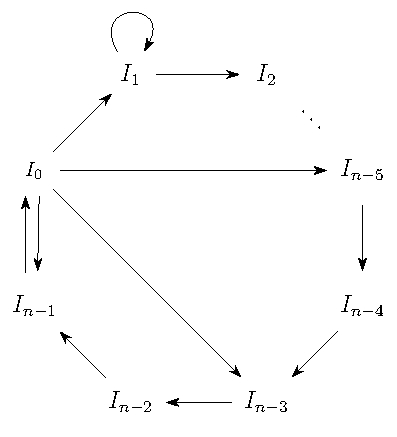
\includegraphics{images/graph_n.pdf}
% \caption[caption za v kazalo]{Dolg caption pod sliko}
  \caption[Primer vektorske slike.]{Relacije pokritja v trditvi~\ref{trd:pokritja} lahko prikažemo z grafom.}
  \label{fig:nkotnik}
\end{figure}

\begin{proof}[Dokaz trditve~\ref{trd:pokritja}]
Dokazovali bomo vsako točko posebej. 

Pri dokazu točke~\ref{trd:pokritja1} bomo dokazali še močnejšo trditev, ki nam bo v pomoč tudi pri dokazu druge točke. Pokazali bomo, da za vsak $j = 0, 1, \dots, n-1$ velja relacija pokritja $I_j \to I_1$.  Za dokaz je dovolj, če se prepričamo, da vsak interval $f(I_j)$ vsebuje točki $x_0$ in $x_1$. V primeru intervala $I_0 = [x_n, x_{n-2}]$ ugotovimo, da obe krajišči $I_0$ ležita na isti strani točke $c$. Lastnost \ref{eq:š4} pove, da krajišče $x_{n-2}$ menja stran, medtem ko lastnost~\ref{eq:š5} pravi, da točka $x_n$ ne menja strani, zato točki $f(x_n)$ in $f(x_{n-2})$ ležita na nasprotnih straneh točke $c$. V primeru intervala $I_j$ za $j = 1, 2, \dots, n-1$ upoštevamo lastnost~\ref{eq:š2} in pridemo do zaključka, da krajišči intervala ležita na nasprotnih straneh točke $c$. Lastnost~\ref{eq:š4} pove, da obe krajišči menjata stran. Torej za vsak $j=0, 1, \dots, n-1$ interval $f(I_j)$ vsebuje točke $\mathcal{O}$-cikla, ki ležijo na obeh straneh centra $c$. Zagotovo vsebuje točki $x_0$ in $x_1$ in zato tudi interval $I_1$.

Naj bo $j$ tako naravno število, za katerega velja $1 \leq j \leq n-1$. Interval $J$ vsebuje interval $I_j$ natanko tedaj, ko vsebuje točke $x_0, x_1$ in $x_j$. Želimo pokazati, da interval $f(x_j)$ vsebuje interval $I_{j+1}$. Vemo že, da interval $f(I_j)$ vsebuje točki $x_0$ in $x_1$. Za dokaz točke~\ref{trd:pokritja2} moramo pokazati samo še vsebovanost točke $x_{j+1}$ v intervalu $f(I_j)$.

Za dokaz točke~\ref{trd:pokritja3} moramo pokazati, da so intervali $I_{n-1}, I_{n-3}, \dots$ vsebovani v intervalu $f(I_0)$.  
Ker že vemo, da $f(I_0)$ vsebuje točki $x_0$ in $x_1$, preostane za dokazati še, da vsebuje točke $x_{n-1}, x_{n-3}, \dots$ Zaradi lastnosti~\ref{eq:š2} ležijo vse točke na drugi strani točke $c$ kot točki $x_{n-2}$ in $x_n$. Iz lastnoti~\ref{eq:š3} sklepamo, da je točka $x_{n-1}$ najbolj oddaljena od točke $c$, zato vsak interval, ki vsebuje točke $x_0, x_1$ in $x_{n-1}$, vsebuje tudi vse točke $x_{n-3}, x_{n-5}, \dots$ Pokazati moramo samo še, da interval $f(I_0)$ vsebuje točko $x_{n-1}$. Pri lastnosti~\ref{eq:š4} namesto $j$ pišemo $n-2$ in dobimo vsebovanost $x_{n-1} \in \mathcal{O}_{f(x_j)}$. Iinterval $f(I_n)$ vsebuje točke $x_0, x_1$ in $f(x_j)$, 

\end{proof}


\begin{proof}[Dokaz trditve~\ref{trd:zap-cikel}]
Naj veljajo predpostavke v trditvi~\ref{trd:zap-cikel}. Radi bi pokazali, da ima funkcija $f$ za vsako naravno število $l\triangleleft m$ točko periode $l$. Dokaz bomo razdelili na tri dele. Najprej bomo dokazali izrek za liha števila manjša od $m$, potem za soda števila manjša od $n$ in na koncu še za vsa števila večja od $n$.

Edino liho število $l$ manjše od $m$, za katerega lahko velja $l\triangleleft m$ je število 1. Za $l=1$ uporabimo zanko l1, ki je zanka dolžine 1 in zato elementarna. Torej obstaja točka periode 1 v intervalu $I_1$.

Naravno število $l \leq n \leq m$ je lahko v relaciji $l \triangleleft m$ samo, če je sodo. Za vsako sodo število $l \leq n$ lahko iz slike~\ref{fig:nkotnik} izpišemo $l$-zanko:
$$I_0\to I_{n-(l-1)} \to I_{n-(l-2)} \to \cdots \to I_{n-2} \to I_{n-1} \to I_0.$$
Iz konstrukcije intervalov $I_0, I_1, \dots, I_n$ vemo, da je notranjost intervala $I_0$ disjunktna z intervali $I_{n-(l-1)}, I_{n-(l-2)}, \dots, I_{n-2}, I_{n-1}$. Krajišči intervala $I_0$ imata periodo $m$ in zato ne moreta sledit zanki. Z uporabo leme~\ref{lem:element} ugotovimo, da je $l$-zanka elementarna, zato obstaja točka iz $I_0$, ki ima periodo $l$.

V primeru, ko je $l >n$ iz slike~\ref{fig:nkotnik} razberemo $l$ zanko
$$I_0\to\underbrace{I_1 \to I_1 \to \cdots  \to I_1}_{l - n +1 \text{ ponovitev intervala } I_1} \to I_2 \to \cdots \to I_{n-1} \to I_0.$$
Če je $l=m$, potem lahko izberemo točko $x_0$, ki ima periodo $m$. Predpostavimo, da je $l \neq m$. Podobno kot v prejšnjem primeru je notranjost intervala $I_0$ disjunktna z intervali $I_1, I_2, \dots, I_{n-1}$. Krajišči intervala $I_0$ pa ne moreta slediti zanki, saj imata periodo $m$, dolžina zanke pa je različna od $m$. Zopet lahko s pomočjo leme~\ref{lem:element} sklepamo, da je $l$-zanka elementarna, kar zagotavlja obstoj točke iz $I_0$, ki ima periodo $l$.
\end{proof}

%#############  KONSTRUKCIJA ŠTEFANOVEGA ZAPOREDJA ##############
\section{Konstrukcija Štefanovega zaporedja} \label{konssz}

\begin{trditev}
Cikel, ki vsebuje vsaj dve točki, vsebuje Štefanovo zaporedje, če vsaj ena točka ne menja strani.
\end{trditev}
\begin{proof}
Naj bo $m$ naravno število večje ali enako $2$ in naj bo $\mathcal{O}$ cikel sestavljen iz $m$ različnih točk. Naj bo množica $\mathcal{M}$ največji tak $\mathcal{O}$-interval, ki vsebuje točki $p$ in $q$, da vsaka točka cikla $\mathcal{O}$, ki je vsebovana v $\mathcal{M}$ menja stran. To pomeni, da za poljubno točko $x \in \mathcal{M} \cap \mathcal{O}$ vse točke iz množice $\mathcal{O}_x$ menjajo stran. Če želimo konstruirati Štefanovo zaporedje, bomo Definiramo množico $\mathcal{S} \subset \mathcal{O}$, ki vsebuje vse kandidate za 


\begin{figure}[h]
  \centering
  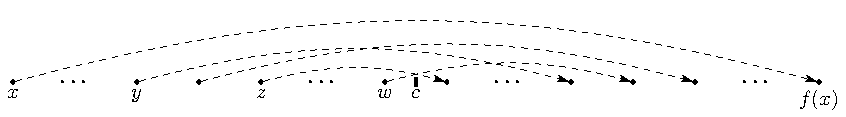
\includegraphics{images/mnozica_S.pdf}
% \caption[caption za v kazalo]{Dolg caption pod sliko}
  \caption[Primer vektorske slike.]{Relacije pokritja v trditvi~\ref{trd:pokritja} lahko prikažemo z grafom.}
  \label{fig:S}
\end{figure}

\begin{figure}[h]
  \centering
  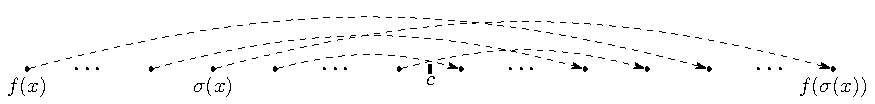
\includegraphics{images/sigma.pdf}
% \caption[caption za v kazalo]{Dolg caption pod sliko}
  \caption[Primer vektorske slike.]{Relacije pokritja v trditvi~\ref{trd:pokritja} lahko prikažemo z grafom.}
  \label{fig:sigma}
\end{figure}

\begin{lema}
Če obstaja taka točka $x \in \mathcal{S}$, za katero je $\sigma^2(x) \in \mathcal{O}_x$, potem vse točke cikla $\mathcal{O}$ menjajo stran.
\end{lema}
\begin{proof}
Če želimo, da je $\sigma^2(x)$ definiran in da leži v $\mathcal{O}_x$, morajo $x$, $y \:= \sigma(x)$ in $z := \sigma(y) = \sigma^2(x)$ vsi ležati v množici $\mathcal{S}$.
\end{proof}
\end{proof}

\begin{trditev}
Naj bo $m$ naravno število večje od 2. Če $m$-cikel vsebuje točko, ki ne menja strani, potem za vsako naravno število $l$, za katero velja $l \triangleleft m$ obstaja elementarna $\mathcal{O}$-vsiljena $l$-zanka $\mathcal{O}$-intervalov in zato tudi točka s periodo $l$.
\end{trditev}
 %#############  DOKAZ IZREKA ŠARKOVSKEGA ##############
\section{Dokaz izreka Šarkovskega}

\begin{trditev}
Naj bosta $m$ in $l$ naravni števili v relaciji $m \triangleleft l$ in naj bo $\mathcal{O}$ $m$-cikel. Potem obstaja $\mathcal{O}$-vsiljena elementarna $l$-zanka $\mathcal{O}$-intervalov in posledično točka s periodo $l$.
\end{trditev}

\begin{proof}
Izrek bomo dokazali s pomočjo indukcije na število $m$. Če je $m=1$, je trditev avtomatično izpolnjena, saj 
\end{proof}

%#############  REALIZACIJSKI IZREK ŠARKOVSKEGA ##############
\section{Realizacijski izrek Šarkovskega}\label{sec:realizacija}
Daljši in bolj zapleten del dokaza izreka Šarkovskega je za nami. Sedaj moramo dokazati še drugi del, ki pravi:
\begin{izrek}
Naj bo $I \subseteq \R$ povezana podmnožica realnih števil. Vsak rep $\mathcal{T}$ ureditve Šarkovskega je množica period za neko zvezno funkcijo $f:I \to I$.
\end{izrek}
\begin{proof}
Izrek bomo dokazali tako, da bomo za vsak rep $\mathcal{T}$ poiskali funkcijo, katere množica period je enaka repu $\mathcal{T}$. Pri iskanju primerne funkcije si bomo pomagali z družino odrezanih šotorskih funkcij. Družino odrezanih šotorskih funkcij definiramo tako, da za vsako realno število $h \in [0, 1]$ definiramo funkcijo:
\begin{equation*} %\label{eq1}
\begin{split}
T_h &:  [0, 1] \to [0, 1] \\ 
T_h &: x \mapsto \min \left(h, 1- 2 \left|x-\frac{1}{2} \right|\right)
\end{split}
\end{equation*}
Ekvivalentno in mogoče lažje predstavljivo lahko predpis funkcije zapišemo na naslednji način:
\begin{equation*} %\label{eq1}
T_h(x) = \min(2x, 2-2x, h).
\end{equation*}
Najprej bomo pokazali, da obstaja funkcija, ki ima samo periodo 1. To je funkcija $T_0$. Hitro vidimo, da je za vsak $x\in [0, 1]$ vrednost funkcije $T_h$ enaka 0, zato je 0 tudi edina periodična točka za to funkcijo. Točka 0 je fiksna točka, zato je njena perioda enaka 1.
Obravnavajmo funkcijo $T_1$. Dokazali bomo, da je vsako naravno število $n$ perioda funkcije $T_1$. To najlažje dokažemo tako, da poiščemo cikel dolžine 3 in s pomočjo izreka XXX sklepamo, da ima funkcija $T_1$ vse periode. Vsaka točka ki ima za funkcijo $T_1$ periodo 3 je fiksna točka funkcije $T_1^3$, zato si poglejmo fiksne točke funkcije $T_1^3$. Iz grafa razberemo, da ima funkcija $T_1^3$ 8 fiksnih točk. Točki 0 in $\frac{2}{3}$ sta fiksni točki funkcije $T_1$, točke $\frac{2}{7}, \frac{4}{7}$ in $\frac{6}{7}$ tvorijo 3-cikel. Prav tako tvorijo 3-cikel točke  $\frac{2}{9}, \frac{4}{9}$ in $\frac{8}{9}$. S pomočjo izreka XXX ugotovimo, da funkcija $T_1$ vsebuje točke vseh period, saj vsebuje točko periode 3.
\begin{lema}
Če je $\mathcal{O} \subseteq [0, h]$ cikel za funkcijo $T_1$, je tudi cikel za funkcijo $T_h$.
Če je $\mathcal{O} \subseteq [0, h)$ cikel za funkcijo $T_h$, je cikel tudi za funkcijo $T_1$.
\end{lema}
\begin{proof}
Funkciji $T_1$ in $T_h$ se razlikujeta samo v tistih točkah $x$, za katere je $T_1(x) > h$. V vseh ostalih točkah, sta funkciji enaki. Privzemimo, da je $\mathcal{O} \subset [0, h]$ cikel za funkcijo $T_1$. To pomeni, da za vsako točko $x \in \mathcal{O}$ velja $T_1(x) \leq h$. Torej velja $T_1(x)=T_h(x)$, kar pomeni, da je $\mathcal{O}$ tudi cikel za funkcijo $T_h$. 
Denimo, da je $\mathcal{O} \subset [0, h)$ cikel za funkcijo $T_h$. Torej je za vsako točko $x$ cikla $\mathcal{O}$ slika $T_h(x)$ manjša od $h$. Velja, da je tudi funkcija točka $T_1(x)$ manjša od $h$. To pomeni, da sta vrednosti funkcij $T_1$ in $T_h$ v $x$ enaki. Ker to velja za vsako točko cikla $\mathcal{O}$, je $\mathcal{O}$ tudi cikel za funkcijo $T_1$.
\end{proof}
V drugem primeru trditev z zaprtim intervalom ne drži, saj ne moremo narediti sklepa, da iz neenakosti $t_h(x) \leq h$ sledi neenakost $T_1(x) \leq h$. To si lahko pogledamo tudi na primeru
\begin{primer}
Presečišča funkcije $T_{0,88}^3$ s simetralo lihih kvadrantov predstavljajo kandidate za periodične funkcije. Iz slike razberemo presečišče $(\frac{6}{25}, \frac{6}{25})$, kar pomeni, da je točka $\frac{6}{25}$ periodična točka za funkcijo $T_{0,88}$. Z iteracijami funkcije $T_{0,88}$ na točki $\frac{6}{25}$ dobimo 3-cikel $\mathcal{O} = \left\{ \frac{6}{25}, \frac{12}{25}, \frac{22}{25} \right\}$. Iz grafa funkcije $T_1^3$ vidimo, da točka $\frac{6}{25}$ ni fiksna točka funkcije $T_1^3$ in zato ne more biti točka periode 3 za funkcijo $T_1$. Cikel $\mathcal{O}$ res ni cikel za funkcijo $T_1$.
\end{primer}

\end{proof}

$$h: \N \to [0, 1], h(m) := \min\{\max \mathcal{O}: \mathcal{O}\text{ je }m\text{-cikel funkcije }T_1 \}$$

\begin{lema}
Naj bosta $m$ in $n$ naravni števili, ki sta v relaciji $m \triangleleft n$. Potem velja ekvivalenca:
$$h(m) \triangleleft h(n) \iff m \triangleleft n.$$
\end{lema}
\begin{dokaz}
Dokaz...
\end{dokaz}

\begin{figure}[h]
  \centering
  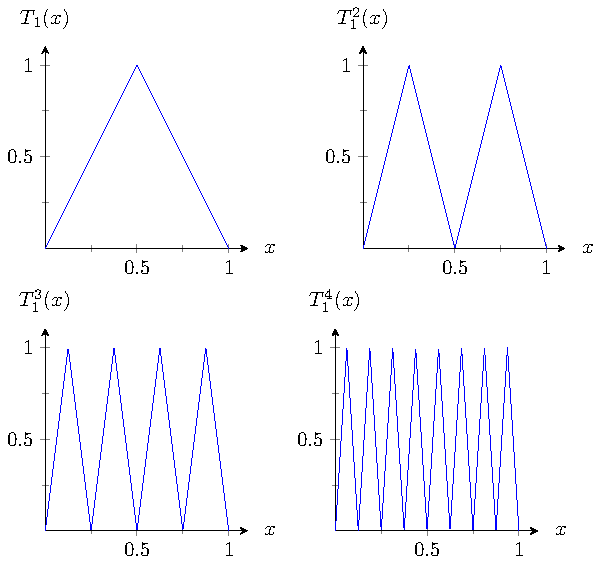
\includegraphics{images/funkcija_T1.pdf}
% \caption[caption za v kazalo]{Dolg caption pod sliko}
  \caption[Primer vektorske slike.]{Relacije pokritja v trditvi~\ref{trd:pokritja} lahko prikažemo z grafom.}
  \label{fig:T1}
\end{figure}

\begin{figure}[h]
  \centering
  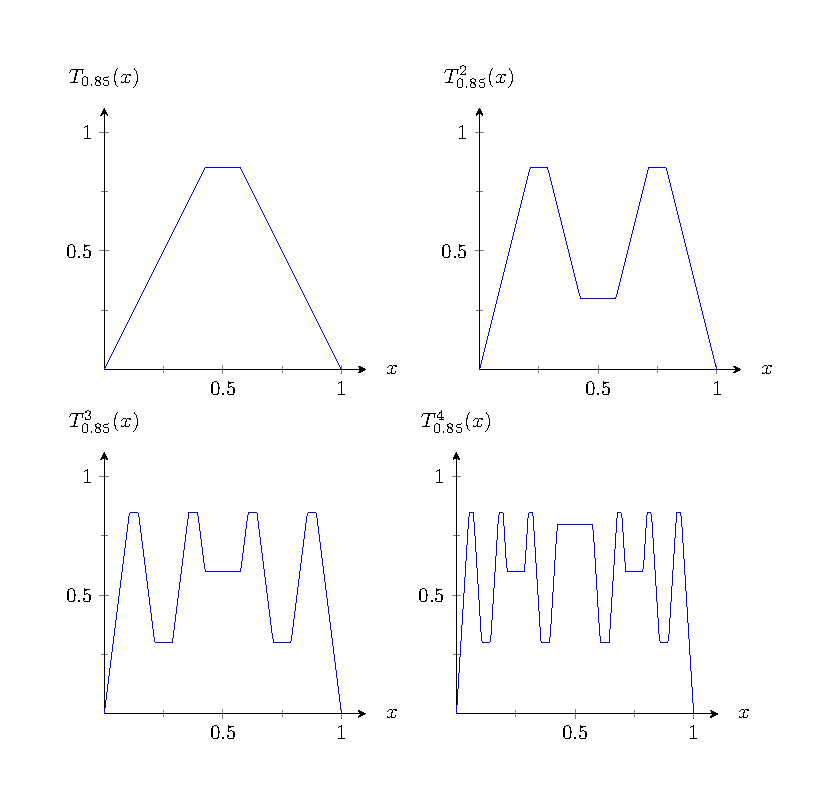
\includegraphics{images/odrezana_funkcija.pdf}
% \caption[caption za v kazalo]{Dolg caption pod sliko}
  \caption[Primer vektorske slike.]{Relacije pokritja v trditvi~\ref{trd:pokritja} lahko prikažemo z grafom.}
  \label{fig:nkotnik}
\end{figure}
%#############  IZREK ŠARKOVSKEGA Z ##############
\section{Prostor sharkovskega}

%#############  IZREK ŠARKOVSKEGA Z ##############
\section{Linearni kontinuum je prostor šarkovskega}






% Literatura:
% Primer navajanja na http://www.fmf.uni-lj.si/storage/24240/LiteraturaM.pdf,
% ampak bi moral stil poskrbeti za vse. Reference se uredijo po abecedi.
% Če nobena izbira izmed @book, @atricle,... ni ok, potem se lahko vse napiše v
% @misc pod note={} in deluje tako kot normalen LaTeX.
% Komentar v bib datoteki se naredi samo s parom { }
% Za urejanje literature avtor priporoča program Jabref, ki zna tudi avtomatsko
% okrajšati imena revij. Za pravilno sortiranje vnosov brez avtorja, uporabite
% polje key={ }, kot v primeru.
% V primeru napak ustvarite issue na GitHubu ali pišite na jure.slak@fmf.uni-lj.si.
\cleardoublepage                           % na desni strani
\phantomsection                            % da prav delujejo hiperlinki
\addcontentsline{toc}{section}{\bibname}   % dodajmo v kazalo
\bibliographystyle{fmf-sl}                 % uporabljen stil je v datoteki fmf-sl.bst, na voljo tudi angleška verzija
%\bibliography{\literatura}                 % literatura je v datoteki, definirani na začetku
% TeXStudio zmede \ zgoraj, tako da lahko notri napišeš dejansko ime .bib datoteke, če ti
% ne delajo predlogi citatov.

% Za stvarno kazalo
\cleardoublepage                           % na desni strani
\phantomsection                            % da prav delujejo hiperlinki
\addcontentsline{toc}{section}{\indexname} % dodajmo v kazalo
\printindex

\end{document}


